\section{Laser-camera triangulation technology}
\label{sec:lctt}
In computer vision, the term \textit{triangulation} refers to the ability to determine a 3D point in the world, through its projections in two or more image planes. Usually the expression ``laser triangulation'' has become a synonym for a system that measures distances using a sensor and a laser. In this thesis, the terms \textit{laser triangulation}, ``\textit{Sheet Of Light}'' (\acs{SOL}), or \textit{light stripe triangulation} will be used as synonyms even though this is not entirely correct, because of the type of laser projector used. Afterwords we will consider only laser stripes. \\

In a 3D triangulation system the three main components are:
\begin{itemize}
  \item a camera (typically based on CCD or C-MOS sensors);
  \item a laser projector (typically a collimated laser);
  \item a software to process images and accurately translate pixel offsets to height differences.
\end{itemize}
In this systems a laser beam is projected against a target object, while one or more acquisition sensors collect images of scene, as in Figure \ref{fig::triang_config}. The analysis of the laser shape on the images allows to reconstruct the object and make measures on it.
\begin{figure}[t!]
  \centering
  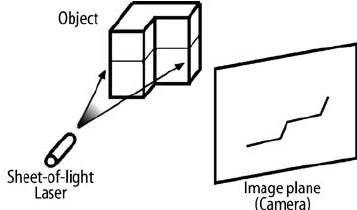
\includegraphics[width=0.5\textwidth]{./images/tech/triang_model_2.png}
  \caption{Example of laser-camera triangulation system}
  \label{fig::triang_config}
\end{figure} \\
Camera and laser are fixed each other and, at the same time, they are rotated at a known angle. In Figure \ref{fig::triang_geoms} the most common system configurations are shown. Each of them has its own pros and cons. \\

\begin{figure}[!b]
  \centering
  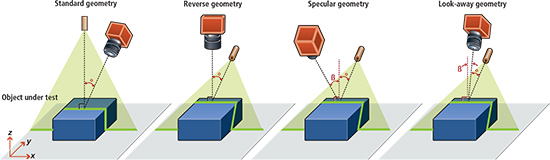
\includegraphics[width=\textwidth]{./images/tech/tech_geometry.jpg}
  \caption{Typical laser-camera configurations}
  \label{fig::triang_geoms}
\end{figure}

\noindent
In the \textit{standard geometry}, the laser line is projected perpendicularly to the $\left( x, y \right)$ nominal plane. This is the simplest configuration because the variation in the target height does not change the coordinate $y$ in the nominal plane. If on the one hand this simplifies system calibration and target shape analysis, resulting in a very fast and accurate system, on the other the camera views the object from a corner by changing the depth of field of the camera. The accommodation of the camera is needed, in order to keep the focus at the height of the object, moreover a test object must be calibrated for accurate measurement results from the system. \\

\noindent
If we switch the positions of projector and camera, we produce the \textit{reverse geometry}. In this case the system is more sensitive to the change in the height of the target, because the laser inclination causes a large shift in the position of the laser line. However these shifts change the value of the $y$ coordinate in the nominal plane, causing a more complex analysis.\\

\noindent
In \textit{specular geometry} configurations, both the projector and camera are placed at non-normal angles compared to the target surface. The placement allows a greater height resolution than the previous configurations, but the camera could see laser specular reflections. This causes noisy effect when acquiring images, such as saturation or blooming. As it happened in reverse geometry, laser inclination caused changes in $y$ coordinates when varying the height of the object. \\

\noindent
The \textit{look-away geometry} was introduced to reduce the laser specular reflections, by placing the projector and the camera at the same side of the target. However, this geometry also reduces height resolution because the camera point of view is very similar to that of the projector. \\

The \textit{standard geometry} is the most used in general purpose systems, thanks to its simplicity of implementation, calibration and use. The \textit{reverse geometry} is typically used in high resolution measurement systems, because of its performances. \textit{Specular geometry} is used, instead, when the accuracy of the system is crucial for the application of interest (such as \acs{WPMS}s), but it can be used only when the surface of the target is dark, highly textured or anyway it is a Lambert's surface. Finally, the \textit{look-away geometry} is suggested any time the target has highly reflective surfaces, such as glass or lucid metals. \\

A common issue of all these configurations is the presence of occlusions. An occlusion occurs when a non-planar target prevents the camera from seeing the laser beam. In Figures \ref{fig:occlusions} the occlusion can be seen from the point of view of the laser (Figure \ref{fig:occlusions_laser}) or from point of view of the camera (Figure \ref{fig:occlusions_camera}). This situation prevents from reconstructing the object properly, so it is often necessary to add one or more cameras or laser-camera pair to have a complete view around the object. In railway wheel analysis occlusions are a common situation to consider.
\begin{figure}[h!]
  \centering
  \begin{minipage}[c]{.50\textwidth}
  	\centering
    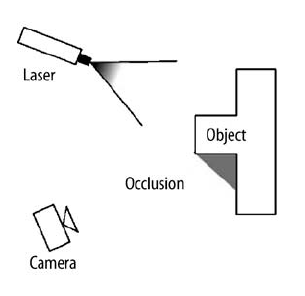
\includegraphics[width=.6\textwidth]{./images/tech/occlusion1.png}
    \subcaption{Laser occlusion}
    \label{fig:occlusions_laser}
  \end{minipage}%
  \begin{minipage}[c]{.50\textwidth}
  	\centering
    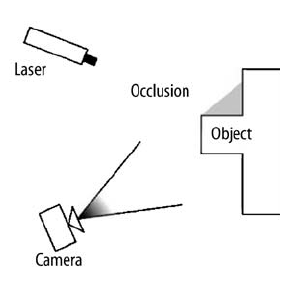
\includegraphics[width=.6\textwidth]{./images/tech/occlusion2.png}
    \subcaption{Camera occlusion}
    \label{fig:occlusions_camera}
  \end{minipage}
  \caption{Examples of different types of occlusions}
  \label{fig:occlusions}
\end{figure}

Another issue due by laser and camera relative positions, is the resolution of the camera. In 2D computer vision, the camera resolution is given by the pixel, according with the relation $resolution = \frac{Field \: of \: view}{sensor \: size}$. This is true only if the entire scene is focusable. In \acs{SOL} systems the angle between camera and laser plane prevents the focus of the entire field of view, that depends on the distance from the lens. We can distinguish three different resolutions described below. Typically, this variance in camera resolution is called \textit{trapezoidal camera resolution}. \\

\noindent
The \textit{depth resolution} is the minimum variation in the target depth appreciable by the camera. It strongly depends on the target distance from the lens and, in particular, on the angle between the projector and the camera. The greater the angle is, the greater is the variation observed in the image plane, caused by the same variation in the 3D space (in metric units). Furthermore it depends also on laser stripe thickness. Many sub-pixel approximation algorithms was developed to reduce the weight of this last factor, and some of this algorithms will be discussed later. \\

\noindent
The \textit{resolution along the laser line} is the ratio between the length of the laser line observed in the camera and the corresponding length in millimeters. As the depth resolution and because of the perspective distortion, this last resolution depends by the object distance from the camera, and it is greater close to the lens. \\

\noindent
The last is the \textit{step between consecutive frames}.
%The last is the \textit{resolution on the motion direction}.
It is present in systems that take many frames of the same object in different positions, using the same laser-camera pair. This ``resolution'' is related to the camera frame-rate and the system motion speed. \\

\noindent
The differences between them will be clearer in the Chapter \ref{ch::model}, where a complete geometric laser-camera triangulation systems model will be presented. However, we can get an idea of these differences by looking at the Figure \ref{fig:tech:resolutions}: the \textit{depth of field} is defined by the extent of the details of the focus areas. \textit{Resolution along the laser line} is given by the details appreciable by the laser itself. Finally, the tape speed and the number of captured images of the same object, define the \textit{capture step}.
  \begin{figure}[t!]
    \centering
    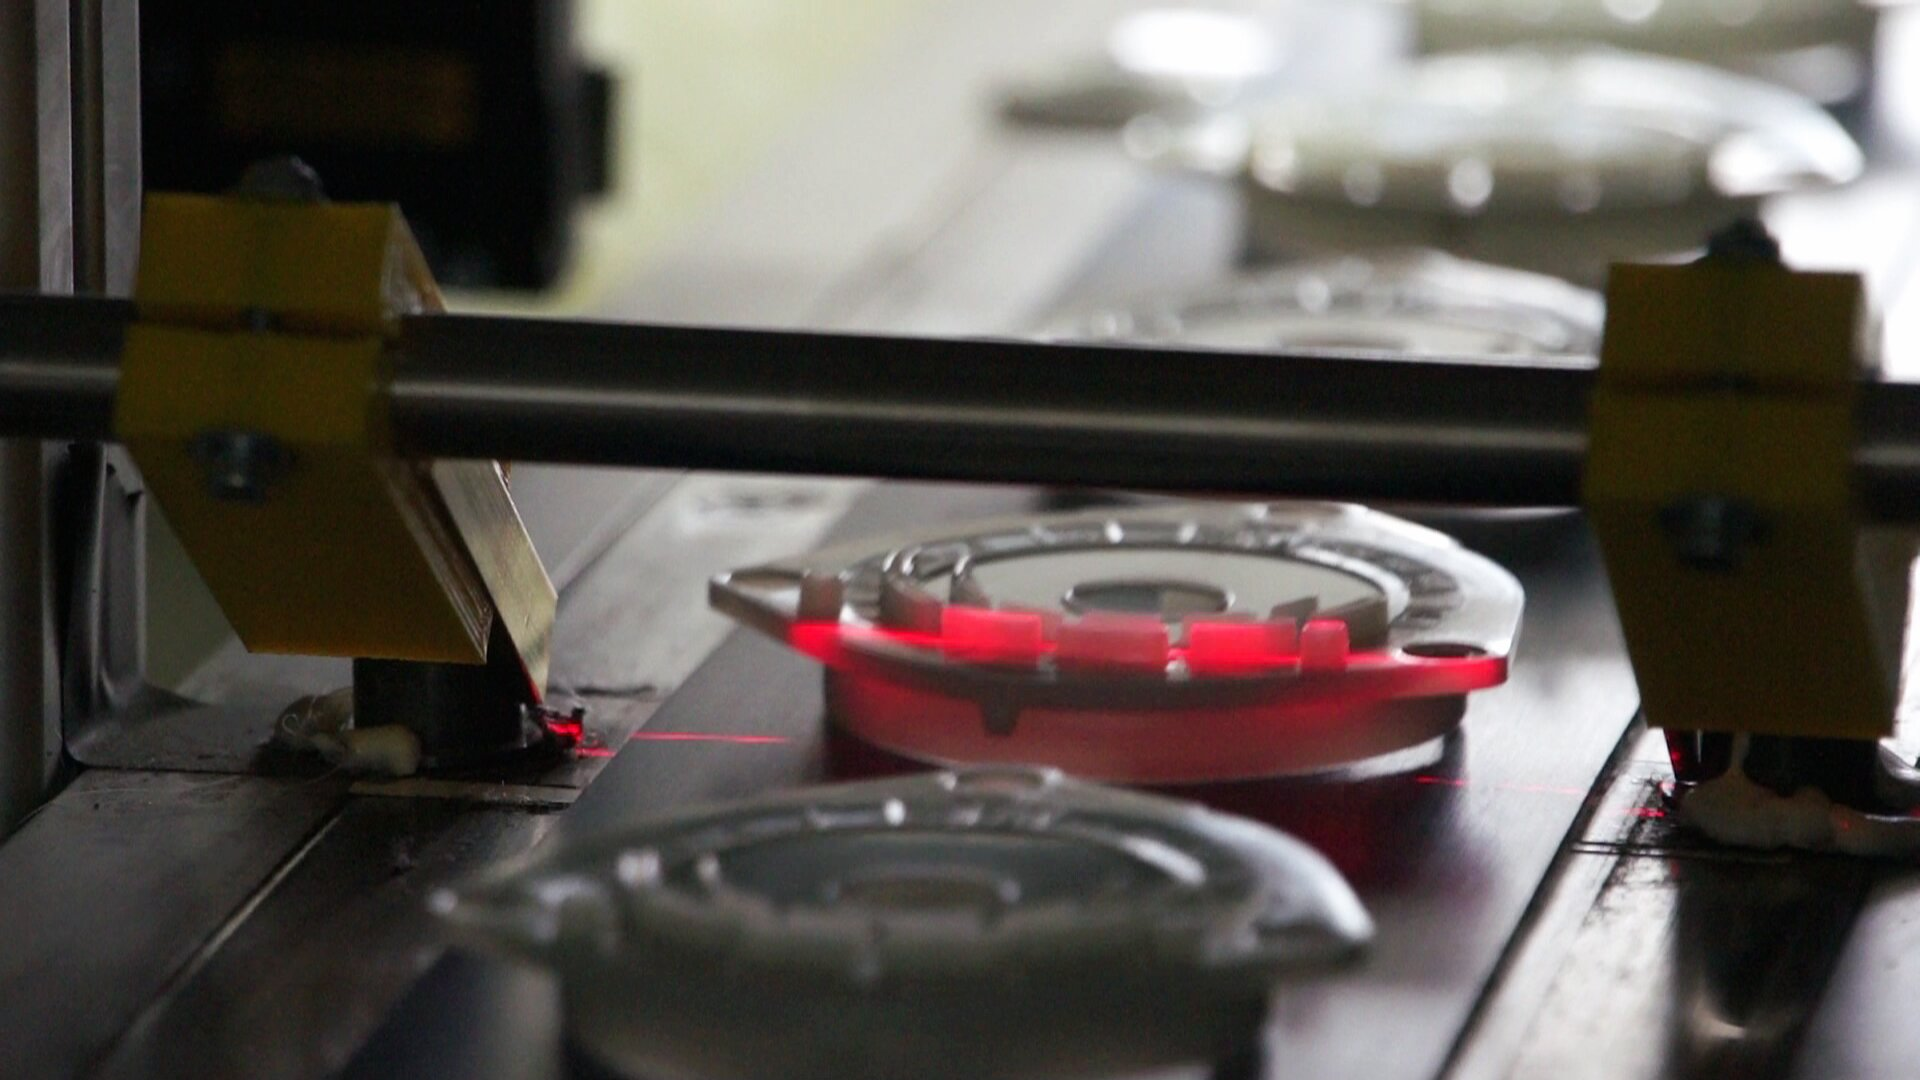
\includegraphics[width=0.8\textwidth]{./images/tech/resolutions.JPG}
    \caption{Representation of the different resolutions of a laser triangular system (property of \url{www.stemmer-imaging.co.uk}).}
    \label{fig:tech:resolutions}
  \end{figure}


% Siti di riferimento:
% http://www.vision-systems.com/articles/print/volume-20/issue-6/features/understanding-laser-based-3d-triangulation-methods.html
% http://www.aqsense.com/docs/docu_3dexpress/limits3D.html
% http://www.aqsense.com/docs/theory3D.pdf
% http://pages.stemmer-imaging.de/techforum-download/pdf/Aqsense_Understanding-and-solving-challenges-in-3D-laser-triangulation-systems_EN.pdf
% http://www.imaginasrl.it/scanner-laser.html
